\documentclass{beamer}
\usepackage{algorithm}
\usepackage{algorithmic}
\usepackage{listings}
\usepackage{xcolor}
\usepackage{color}

\usepackage[absolute,overlay]{textpos}
\usepackage{graphicx}

\newcommand{\defeq}{\stackrel{\triangle}{=}}

\newcommand{\N}{\mathbb{N}}
\newcommand{\tr}{\mbox{tr}}
\newcommand{\bg}{\widehat{\nabla}F}
\newcommand{\fraction}[2]{\textstyle\frac{#1}{#2}} 
\DeclareMathOperator{\sgn}{sgn} 

\newcommand{\hilight}[1]{\setlength{\fboxsep}{0pt}\colorbox{yellow}{#1}}

\newtheorem{defn}{Definition}[section]
\newtheorem{thm}{Theorem}[section]
\newtheorem{prop}{Proposition}
\newtheorem{conjecture}[thm]{Conjecture}
\newtheorem{lem}[thm]{Lemma} 
\newtheorem{cor}[thm]{Corollary}

\lstset{basicstyle=\scriptsize\ttfamily,breaklines=true}
\lstset{framextopmargin=50pt}

\usetheme{Madrid}

\begin{document}

\title[EGR]{EGR: An Evolving Gradient Resampling Method for Stochastic Optimization}
\author[Solntsev, Stefan] % (optional, for multiple authors)
{Stefan Solntsev \and Jorge Nocedal \and Figen Oztoprak \and Richard Byrd}
\institute[Northwestern University]

\begin{frame}
	\titlepage
\end{frame}

\begin{frame}
	\frametitle{Problem Setting}
	\begin{block}{}
	The optimization problem of interest is
	\begin{equation*}
		\label{prob}
		\min F(\theta) = \mathbb{E}[ f(Z;\theta)]
	\end{equation*}
	where $Z$ is a random variable with distribution $P$
	\end{block}
	
	\pause
	
	\begin{block}{}
	Given $m$ samples $z_i$, the objective $F$ can be approximated by the deterministic function
	\begin{equation*}
		\label{saa}
 		\hat{F}(\theta) = \frac{1}{m} \sum_{i=1}^{m}  f(z_i;\theta)  =\frac{1}{m} \sum_{i=1}^{m}  f_i(\theta)\approx F(\theta),
	\end{equation*}
	This is a common setting in stochastic optimization and machine learning
	\end{block}
\end{frame}	 

		\begin{frame}
			\frametitle{Algorithms for $F$ and $\hat{F}$}
			\begin{itemize}
	\pause
				\item Deterministic (batch) methods
	\pause
				\item Stochastic Gradient methods [Robbins, Monro 1951]
	\pause 
				\item SAG [Schmidt, Le Roux, Bach 2013]
	\pause
				\item SVRG [Johnson, Zhang 2013]
	\pause
				\item MISO [Mairal 2013]
	\pause
				\item SDCA [Shalev-Schwartz, Zhang 2012]
	\pause
				\item Stochastic versions of deterministic methods: SDA [Nesterov, 1983, 2009], SQN [Byrd, Hansen, Nocedal, Singer 2014], [Bordes
et al. 2009], [Martens 2010]
			\end{itemize}
			\end{frame}
			

		\begin{frame}
			\frametitle{Algorithms for $F$ and $\hat{F}$}
			\begin{itemize}
				\item Deterministic (batch) methods
				\item \colorbox{yellow}{Stochastic Gradient methods} [Robbins, Monro 1951] 
				\item SAG [Schmidt, Le Roux, Bach 2013]
				\item SVRG [Johnson, Zhang 2013]
				\item MISO [Mairal 2013]
				\item SDCA [Shalev-Schwartz, Zhang 2012]
				\item Stochastic versions of deterministic methods: SDA [Nesterov, 1983, 2009], SQN [Byrd, Hansen, Nocedal, Singer 2014], [Bordes
et al. 2009], [Martens 2010]
			\end{itemize}
			\end{frame}
			
			
		\begin{frame}
			\frametitle{Stochastic Gradient method for $F$}

				\begin{block}{Iteration $k$ of SGD}
			\[
		\theta_{k+1}= \theta_k - \alpha_k \nabla_\theta f(z_k;\theta_k)
		\]
		where $z_k$ is a randomly drawn sample from $P$  \\
\end{block}

	
			\begin{itemize}
	\pause
				\item Designed for $F$ 
	
	\pause
				\item Given $m$ samples, SGD can be emulated by drawing from these samples
	
	\pause
				\item In this setting, SGD with a well-tuned step $\alpha_k$ is competitive with the best known methods in the first few epochs
	
	\begin{itemize}
	\pause
		\item An \textit{epoch} is defined as $m$ evaluations of $\nabla_\theta f(z_k;\theta_k)$
	\end{itemize}
	\pause
	
				\item $\alpha_k$ is hard to tune
				\pause
				\item Step has a high variance 
			\end{itemize}
		\end{frame}

		\begin{frame}
			\frametitle{Algorithms for $F$ and $\hat{F}$}
			\begin{itemize}
				\item Deterministic (batch) methods
				\item Stochastic Gradient methods [Robbins, Monro 1951] 
				\item \colorbox{yellow}{SAG} [Schmidt, Le Roux, Bach 2013]
				\item SVRG [Johnson, Zhang 2013]
				\item MISO [Mairal 2013]
				\item SDCA [Shalev-Schwartz, Zhang 2012]
				\item Stochastic versions of deterministic methods: SDA [Nesterov, 1983, 2009], SQN [Byrd, Hansen, Nocedal, Singer 2014], [Bordes
et al. 2009], [Martens 2010]
			\end{itemize}
			\end{frame}
		\begin{frame}
			\frametitle{SAG: Illustration $m=9$}
			\begin{center}
					\includegraphics{sag7.pdf}
			\end{center}
	    \end{frame}

		\begin{frame}
			\frametitle{SAG: Illustration $m=9$}
			\begin{center}
					\includegraphics{sag6.pdf}
			\end{center}
	    \end{frame}

		\begin{frame}
			\frametitle{SAG: Illustration $m=9$}
			\begin{center}
					\includegraphics{sag5.pdf}
			\end{center}
	    \end{frame}

		\begin{frame}
			\frametitle{SAG: Illustration $m=9$}
			\begin{center}
					\includegraphics{sag4.pdf}
			\end{center}
	    \end{frame}

		\begin{frame}
			\frametitle{SAG: Illustration $m=9$}
			\begin{center}
					\includegraphics{sag3.pdf}
			\end{center}
	    \end{frame}

		\begin{frame}
			\frametitle{SAG: Illustration $m=9$}
			\begin{center}
					\includegraphics{sag2.pdf}
			\end{center}
	    \end{frame}

		\begin{frame}
			\frametitle{SAG: Illustration $m=9$}
			\begin{center}
					\includegraphics{sag1.pdf}
			\end{center}
	    \end{frame}
		
		\begin{frame}
			\frametitle{Stochastic Average Gradient method for $\hat{F}(\theta) $}
				\begin{block}{Iteration $k$ of SAG}
 \begin{align*}
   y_i &= \nabla f_i(\theta^k) \quad \mbox{where } i \mbox{ is sampled from } \{1,\ldots,m\} \\
   \hat{g_k} &= \frac{1}{m} \sum_{i=1}^m y_i , \\
   \theta^{k+1} &= \theta^k - \alpha_k \hat{g_k}
 \end{align*}
\end{block}
	
			\begin{itemize}
	\pause
				\item Requires $\{y_1,\ldots,y_m\}$ initialized and stored. 
				
				\begin{itemize}
	\pause
					\item Tricks to initialize $y$ include SGD, SAG-like buildup, a full pass at $\theta_0$
				\end{itemize}
	
	\pause
				\item Works well on $\hat{F}$ (Good training algorithm)
	
	\pause
				\item Shows its strength after many epochs
			\end{itemize}
	\pause
			We want an algorithm with some of these properties that works well on $F$
		\end{frame}
		
		
		
		\begin{frame}
			\frametitle{EGR: Ideas}
			\begin{itemize}
				\item No ambiguous initialization
				
				\item Sample size grows, does not depend on $m$ (Evolving)
	
				\item Old information is stored
	
				\item Old information is renewed (Resampled)
			\end{itemize}
		\end{frame}	 
		
		
	 		\begin{frame}
	 			\frametitle{EGR: Full Algorithm}

		\begin{block}{Iteration $k$ the Evolving Gradient Resampling (EGR) method}
	 	\begin{align*}
		S_k &=  \mbox{sample of } s_k \mbox{ indices from } I_{k}\\
		\mbox{replace } y_i &= \nabla f_i(\theta^k) \mbox{ for all } i \in S_k \\
		U_k &=  \mbox{sample of } u_k \mbox{ indices from }  I_{k}^C\\
		\mbox{compute } y_i &= \nabla f_i(\theta^k) \mbox{ for all } i \in U_k \\
		I_{k+1} &=  I_{k} \cup U_k\\
		\hat{g_k} & = \frac{1}{| I_{k+1} | } \sum_{i \in I_{k+1}} y_i \\ 
	   	\theta^{k+1} &= \theta^k - \alpha_k \hat{g_k}\\
	 	\end{align*}
		\end{block}
		This method is in itself a strategy to fill up the gradient memory from zero.
	 	    \end{frame}
		
		
		
		\begin{frame}
			\frametitle{EGR: Illustration}
			\begin{center}
					\includegraphics{egr11.pdf}
			\end{center}
	    \end{frame}
		\begin{frame}
			\frametitle{EGR: Illustration}
			\begin{center}
					\includegraphics{egr10.pdf}
			\end{center}
	    \end{frame}
		\begin{frame}
			\frametitle{EGR: Illustration}
			\begin{center}
					\includegraphics{egr9.pdf}
			\end{center}
	    \end{frame}
		\begin{frame}
			\frametitle{EGR: Illustration}
			\begin{center}
					\includegraphics{egr8.pdf}
			\end{center}
	    \end{frame}
		\begin{frame}
			\frametitle{EGR: Illustration}
			\begin{center}
					\includegraphics{egr7.pdf}
			\end{center}
	    \end{frame}
		\begin{frame}
			\frametitle{EGR: Illustration}
			\begin{center}
					\includegraphics{egr6.pdf}
			\end{center}
	    \end{frame}
		\begin{frame}
			\frametitle{EGR: Illustration}
			\begin{center}
					\includegraphics{egr5.pdf}
			\end{center}
	    \end{frame}
		\begin{frame}
			\frametitle{EGR: Illustration}
			\begin{center}
					\includegraphics{egr4.pdf}
			\end{center}
	    \end{frame}
		\begin{frame}
			\frametitle{EGR: Illustration}
			\begin{center}
					\includegraphics{egr3.pdf}
			\end{center}
	    \end{frame}
		\begin{frame}
			\frametitle{EGR: Illustration}
			\begin{center}
					\includegraphics{egr2.pdf}
			\end{center}
	    \end{frame}
		\begin{frame}
			\frametitle{EGR: Illustration}
			\begin{center}
					\includegraphics{egr1.pdf}
			\end{center}
	    \end{frame}

		
	 		\begin{frame}
	 			\frametitle{EGR: Full Algorithm}

		\begin{block}{Iteration $k$ the Evolving Gradient Resampling (EGR) method}
	 	\begin{align*}
		S_k &=  \mbox{sample of } s_k \mbox{ indices from } I_{k}\\
		\mbox{replace } y_i &= \nabla f_i(\theta^k) \mbox{ for all } i \in S_k \\
		U_k &=  \mbox{sample of } u_k \mbox{ indices from }  I_{k}^C\\
		\mbox{compute } y_i &= \nabla f_i(\theta^k) \mbox{ for all } i \in U_k \\
		I_{k+1} &=  I_{k} \cup U_k\\
		\hat{g_k} & = \frac{1}{| I_{k+1} | } \sum_{i \in I_{k+1}} y_i \\ 
	   	\theta^{k+1} &= \theta^k - \alpha_k \hat{g_k}\\
	 	\end{align*}
		\end{block}
		This method is in itself a strategy to fill up the gradient memory from zero.
	 	    \end{frame}
		
		
		\begin{frame}
			\frametitle{Examples}
			
			Some choices of growth sequences $s_k$ and $u_k$ 
			
				
			\begin{itemize}
	\pause
				\item $u_k=0$, $s_k=1$, $I_0=\{1,\ldots,m\}$
				\begin{itemize}
					\item SAG
				\end{itemize}
	
	\pause
				\item $u_k=0$, $s_k=m$, $I_0=\{1,\ldots,m\}$
				\begin{itemize}
					\item Batch Gradient Descent
				\end{itemize}
	
	\pause
				\item $u_k=k+1$, $s_k=k$, $I_0=\emptyset$
				\begin{itemize}
					\item Quadratic growth of $|I_k|$
				\end{itemize}
	
	\pause
				\item $u_k=s_k=\left(\frac{r}{r-1}\right)^{k-1}$, $I_0=\emptyset$
				\begin{itemize}
					\item Exponential growth of $|I_k|$
					\item Always replace/sample a fixed percentage of $|I_k|$ at every iteration
				\end{itemize}
	
			\end{itemize}

	    \end{frame}

\begin{frame}
	\frametitle{Numerical Experiments}
	Since $F$ is not available, we split the $m$ datapoints into two sets, and define\\
	
	\pause
	The \textit{training} function $F_{tr} = \frac{1}{m_{tr}} \sum_{i=1}^{m_{tr}}  f_i(\theta) $ 
	\begin{itemize}
		\item We run the optimization algorithms on this function
	\end{itemize}
	
	\pause
	The \textit{testing} function $F_{te} =\frac{1}{m_{te}} \sum_{i=m_{tr}+1}^{m_{tr}+m_{te}}  f_i(\theta) $
	\begin{itemize}
		\item A common way to assess if progress is being made on $F$ 
	\end{itemize}
	
	\pause
Compare EGR with SGD, SAG
	
\end{frame}

		\begin{frame}
			\frametitle{Numerical Experiments: Outline}
			Tested on a few binary and multiclass classification datasets. 
			\begin{itemize}
				\item \textbf{Random} - a randomly generated binary classification data. 50 variables, 1000000 training datapoints. 
				\item \textbf{Alpha}  - a common test set for binary classification. 175000 training points and 501 variables.
				\item \textbf{Speech} - a multiclass classification dataset. 191607 training points, 30315 variables. 
			\end{itemize}
			The loss function is always the cross entropy.
			
     	\end{frame}
		
 
		\begin{frame}
			\frametitle{Rand Problem: Tune to reach best training function value}
			\begin{center}
					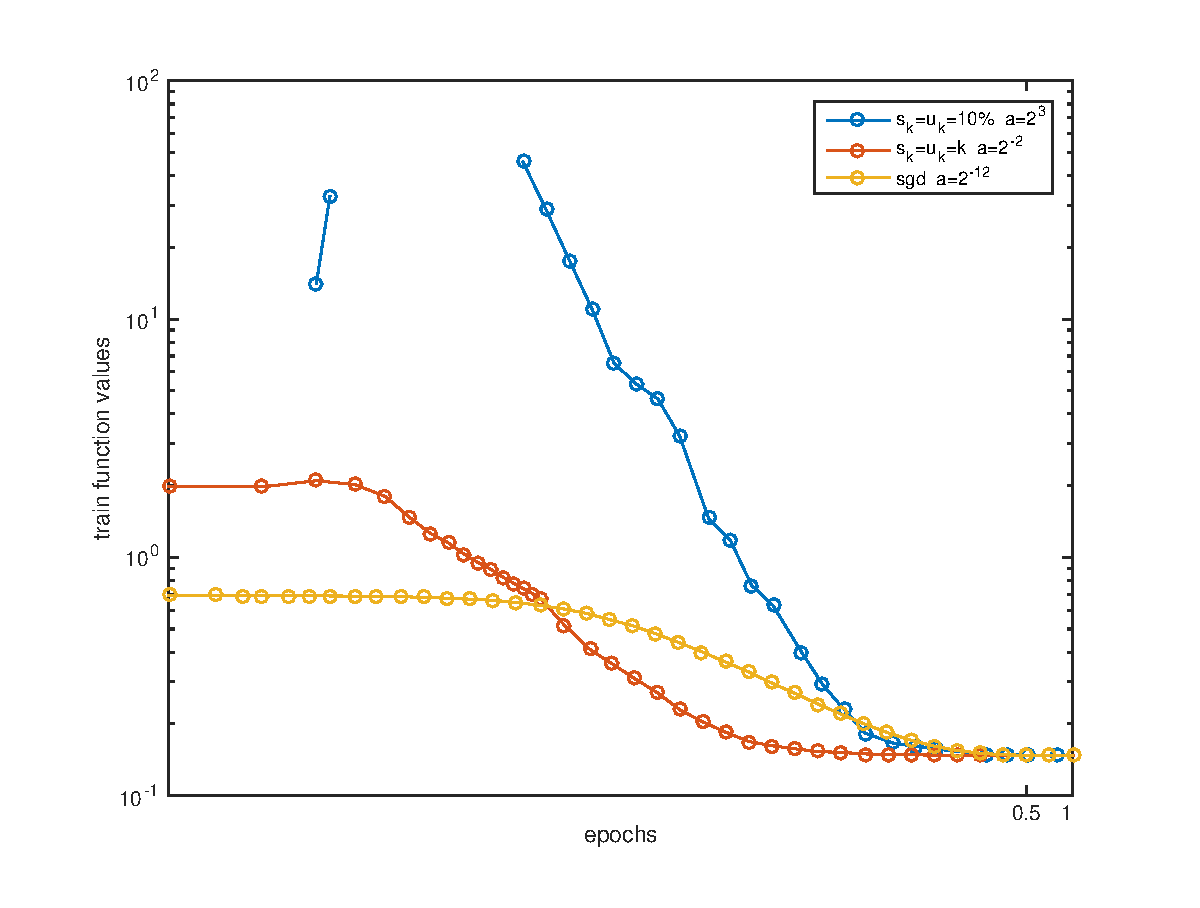
\includegraphics[scale=0.5]{whowins1.eps}
			\end{center}
     	\end{frame}

\begin{frame}
	        \frametitle{Rand Problem: Tune to reach $\hat{F}=0.1514$}
	\begin{center}
			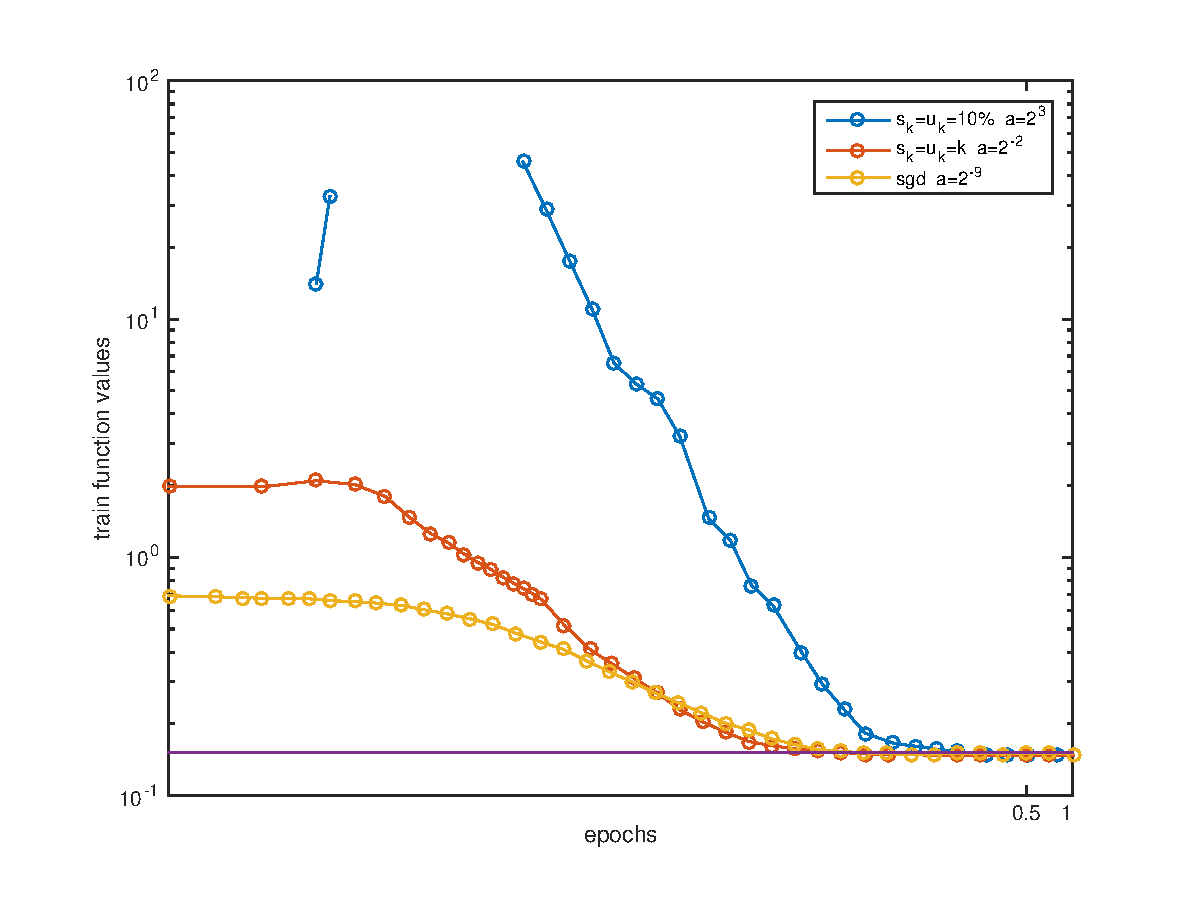
\includegraphics[scale=0.5]{whowins2-1.eps}
	\end{center}
\end{frame}

		\begin{frame}
			\frametitle{Rand Problem: Tune to reach $\hat{F}=0.2291$}
			\begin{center}
					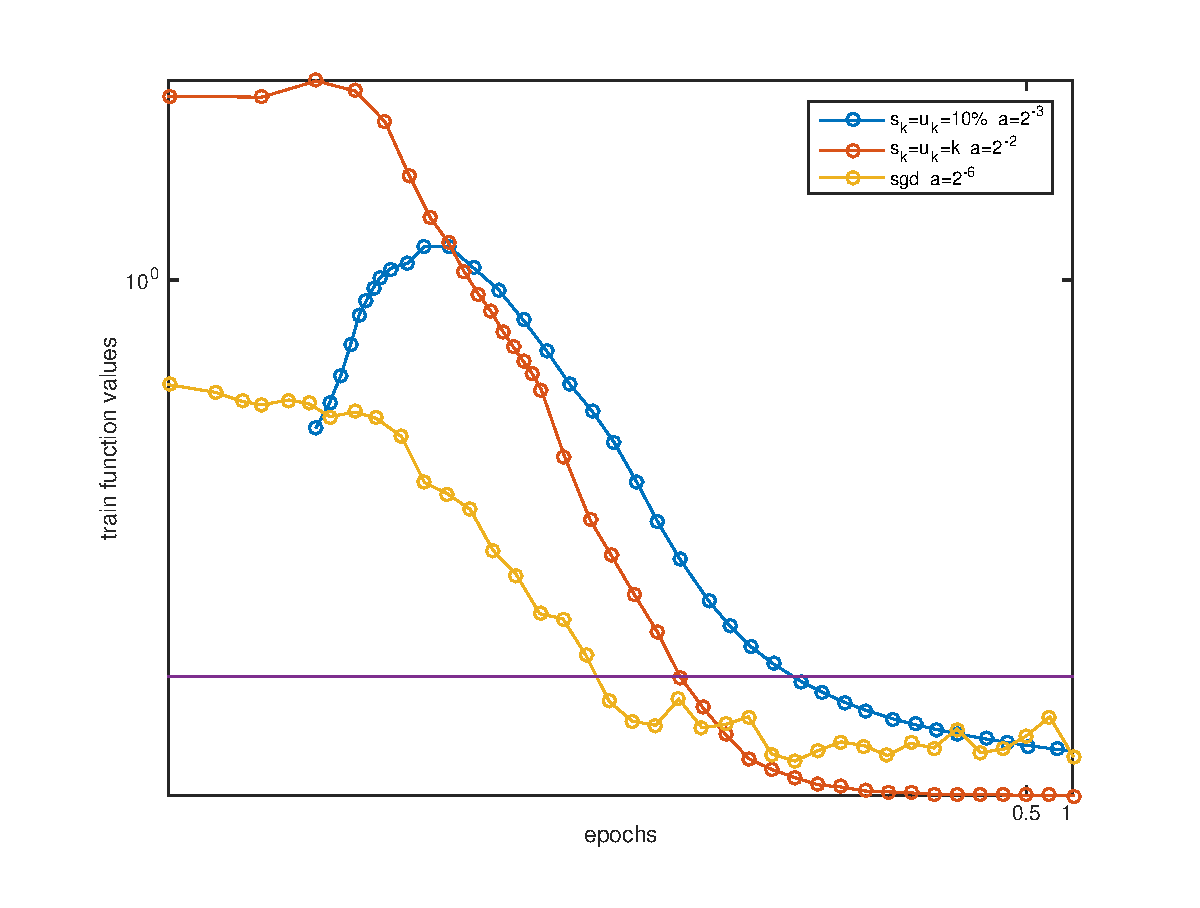
\includegraphics[scale=0.5]{whowins3-1.eps}
			\end{center}
     	\end{frame}
		
		\begin{frame}
			\frametitle{Rand Problem: Compare All SGD steplengths}
			\begin{center}
					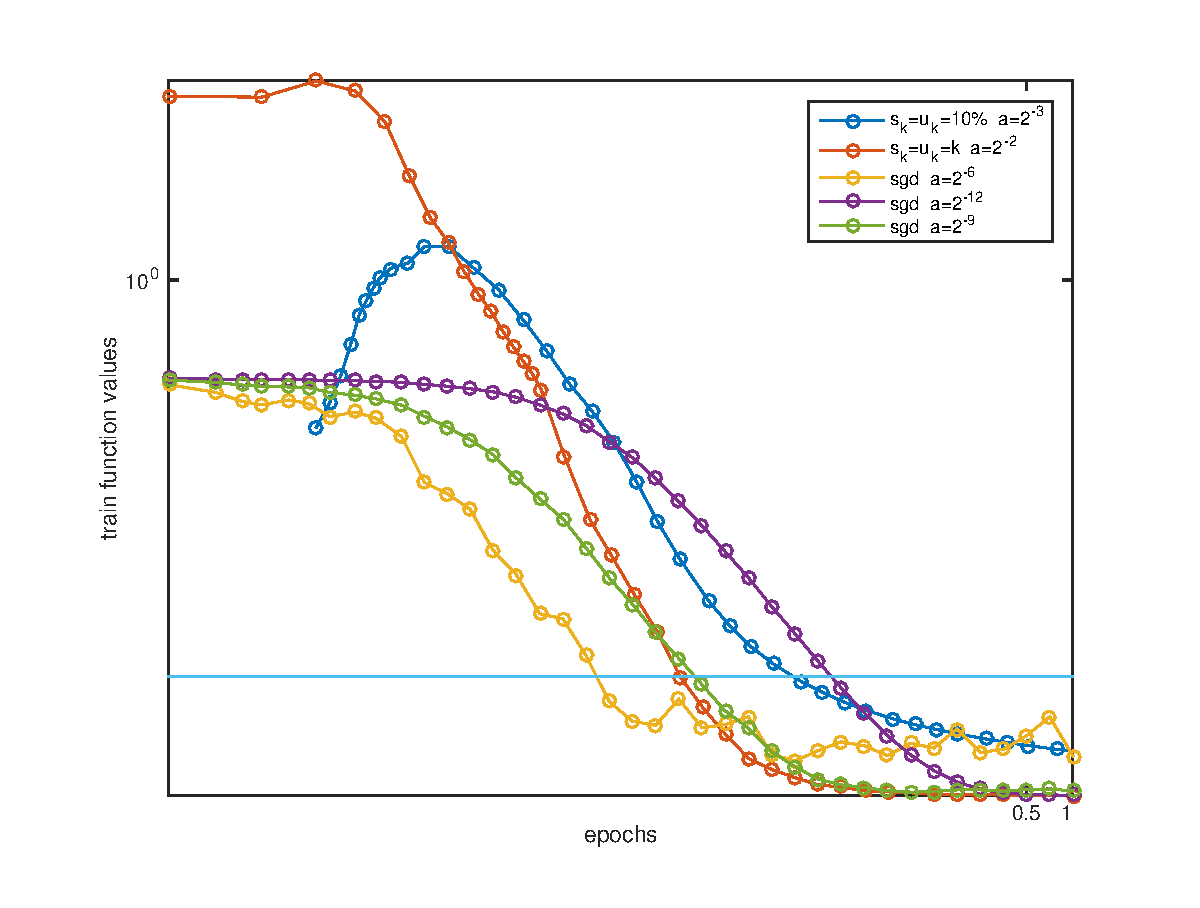
\includegraphics[scale=0.5]{whowins4-1.eps}
			\end{center}
     	\end{frame}
		
		\begin{frame}
			\frametitle{Rand Problem: Gradient Errors}
			\begin{center}
					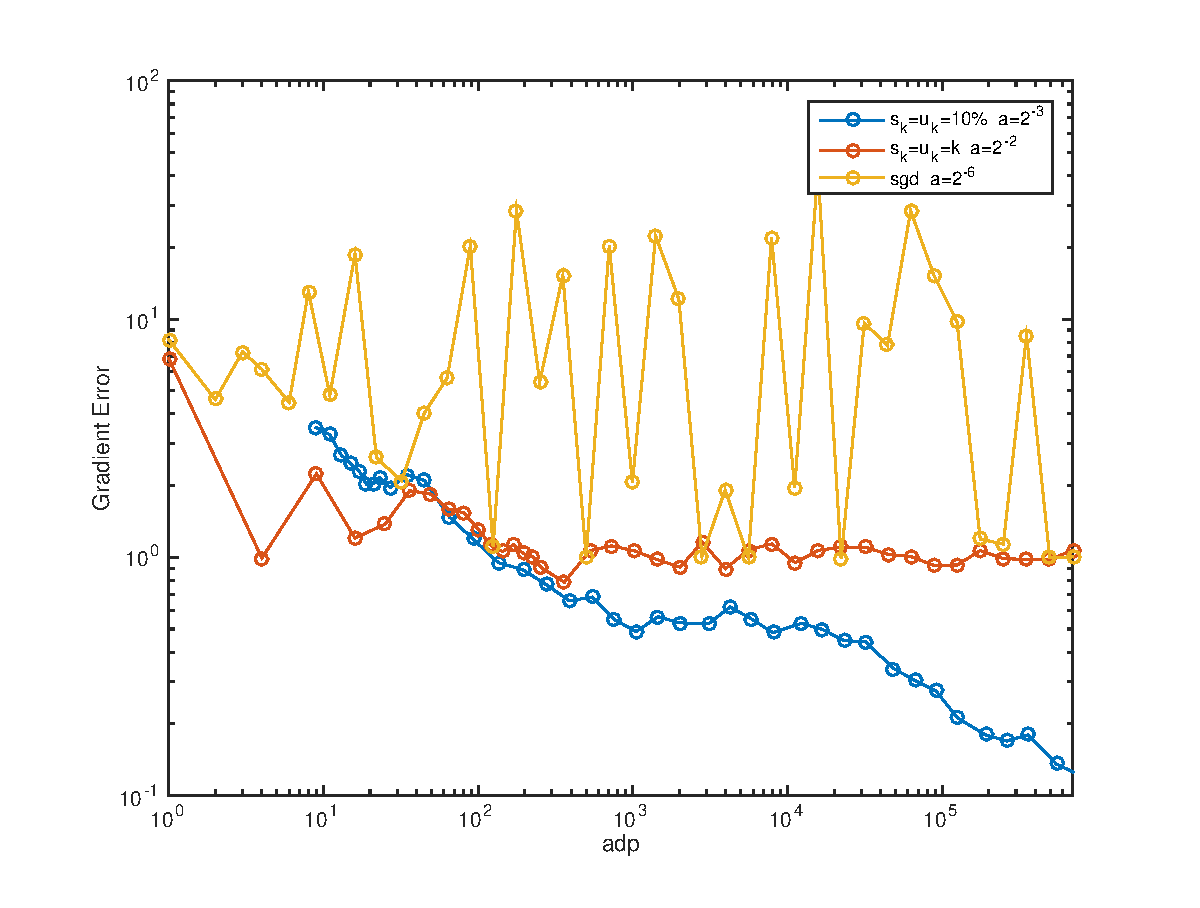
\includegraphics[scale=0.5]{rand-results-gerror.eps}
			\end{center}
     	\end{frame}

\begin{frame}
	\frametitle{Function Values: Alpha}
	\begin{center}
			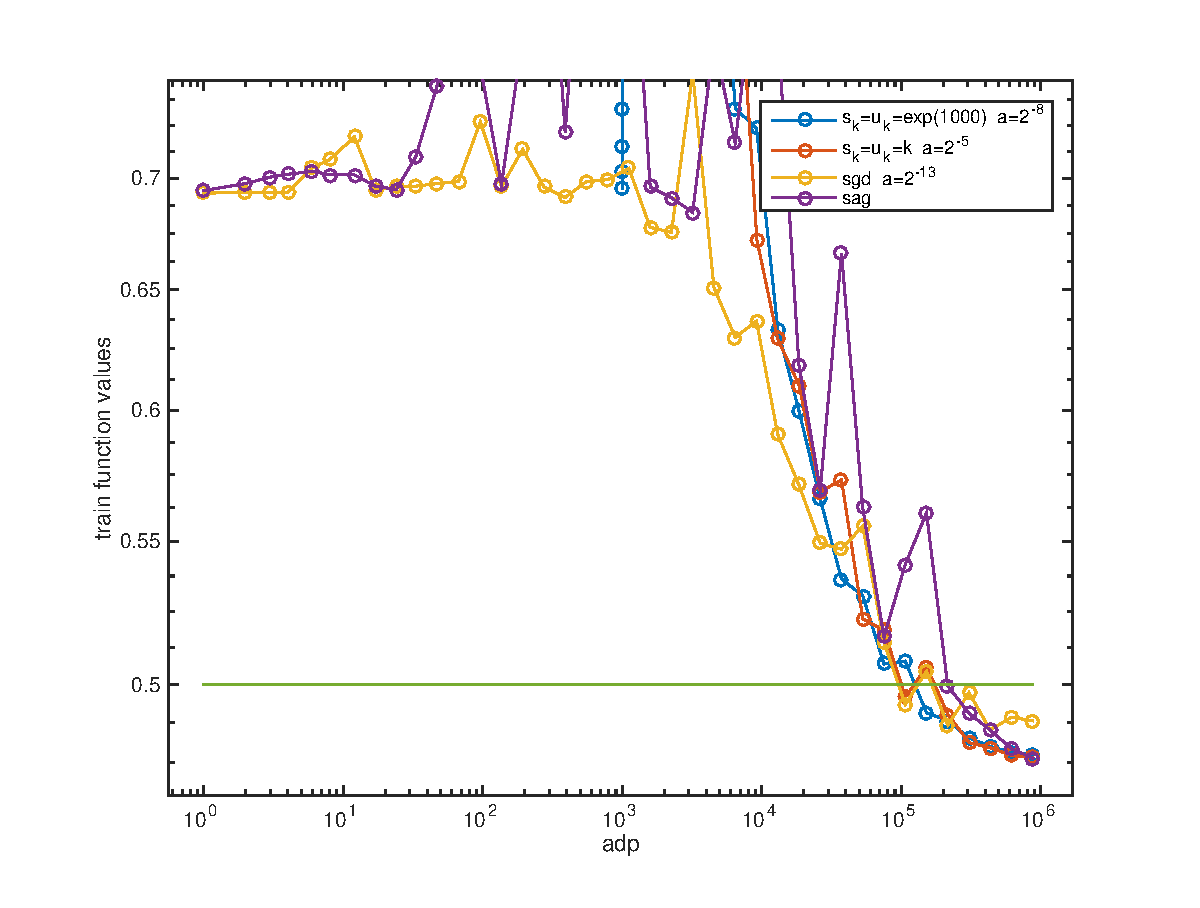
\includegraphics[scale=0.5]{alpha-results-fvals.eps}
	\end{center}
\end{frame}


\begin{frame}
	\frametitle{Gradient Norms: Speech}
	\begin{center}
			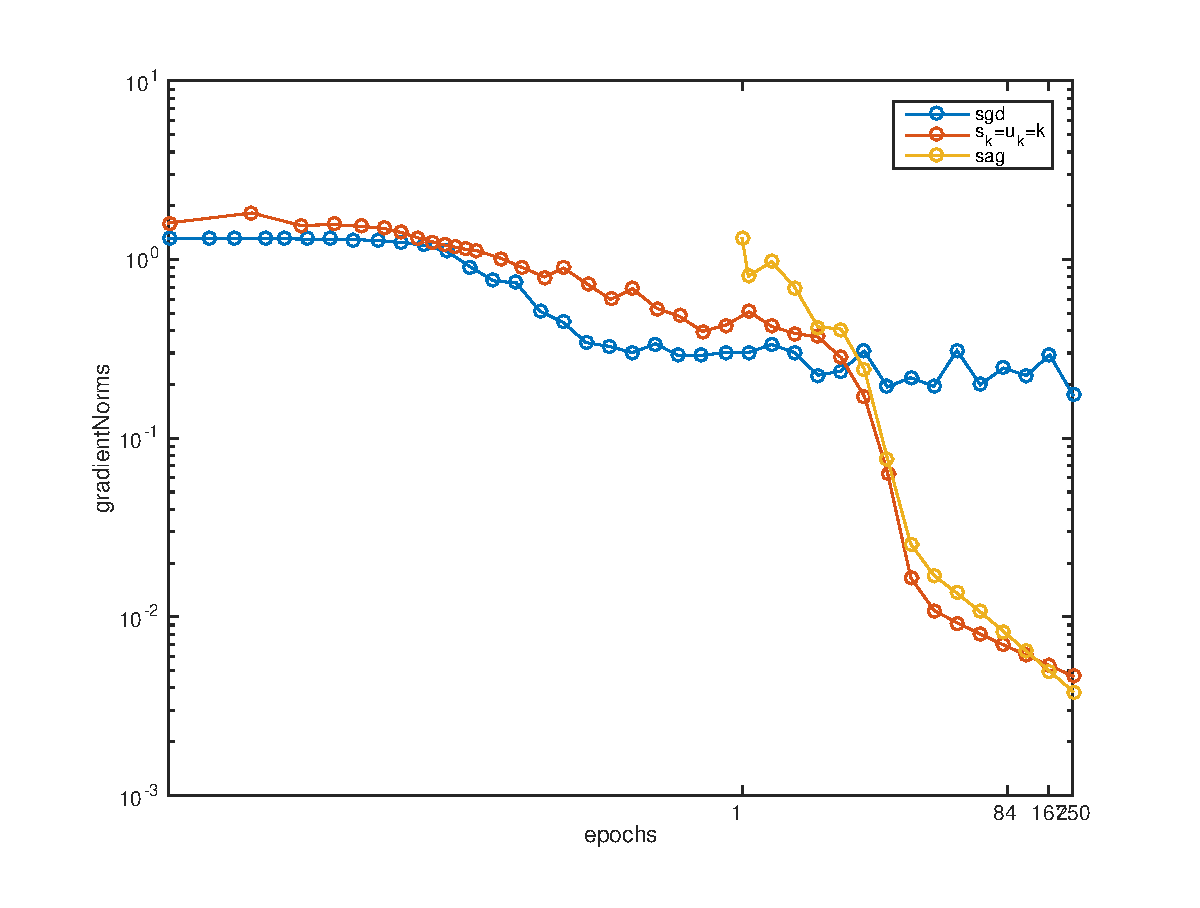
\includegraphics[scale=0.5]{figA.eps}
	\end{center}
\end{frame}

\begin{frame}
	\frametitle{Gradient Norms: Speech}
	\begin{center}
			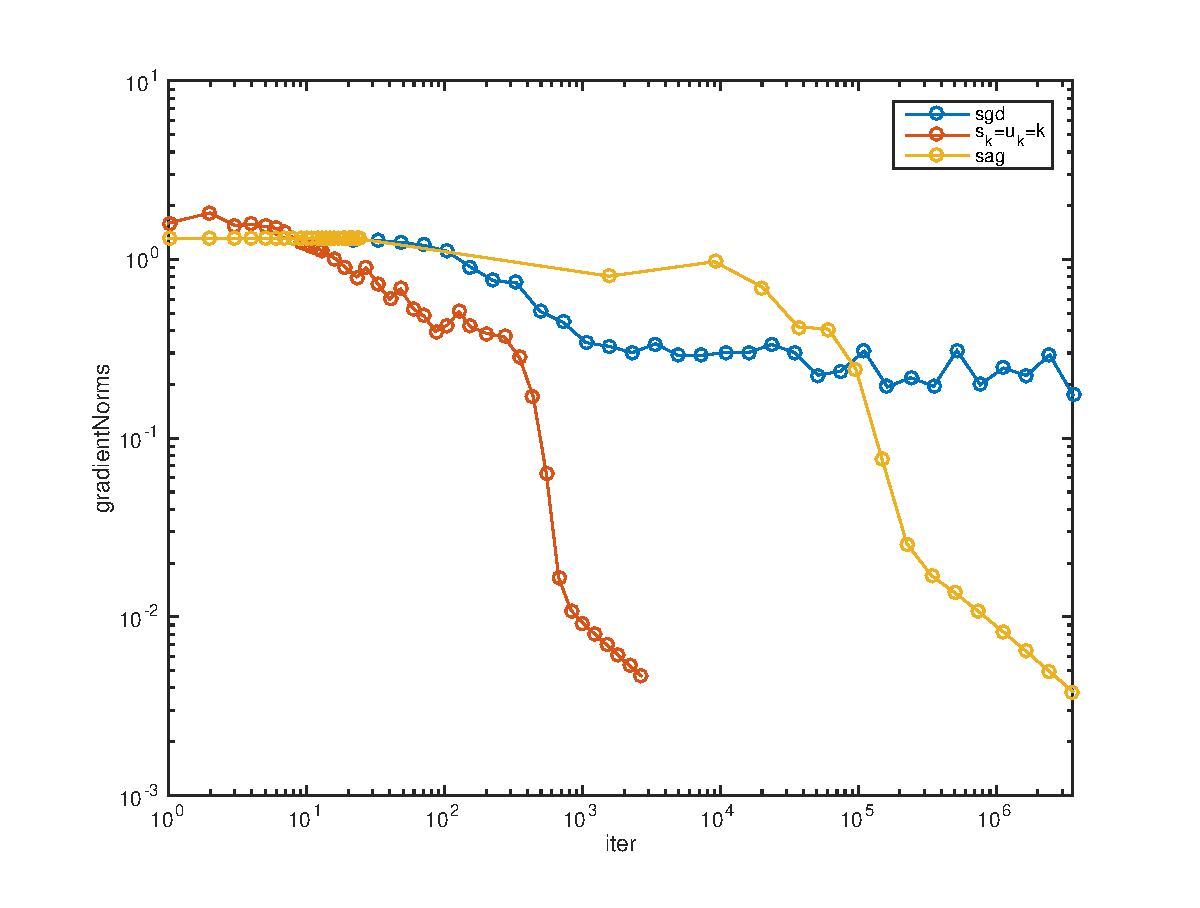
\includegraphics[scale=0.5]{kk.eps}
	\end{center}
\end{frame}

\begin{frame}
	\frametitle{Test Function Values: Speech}
	\begin{center}
			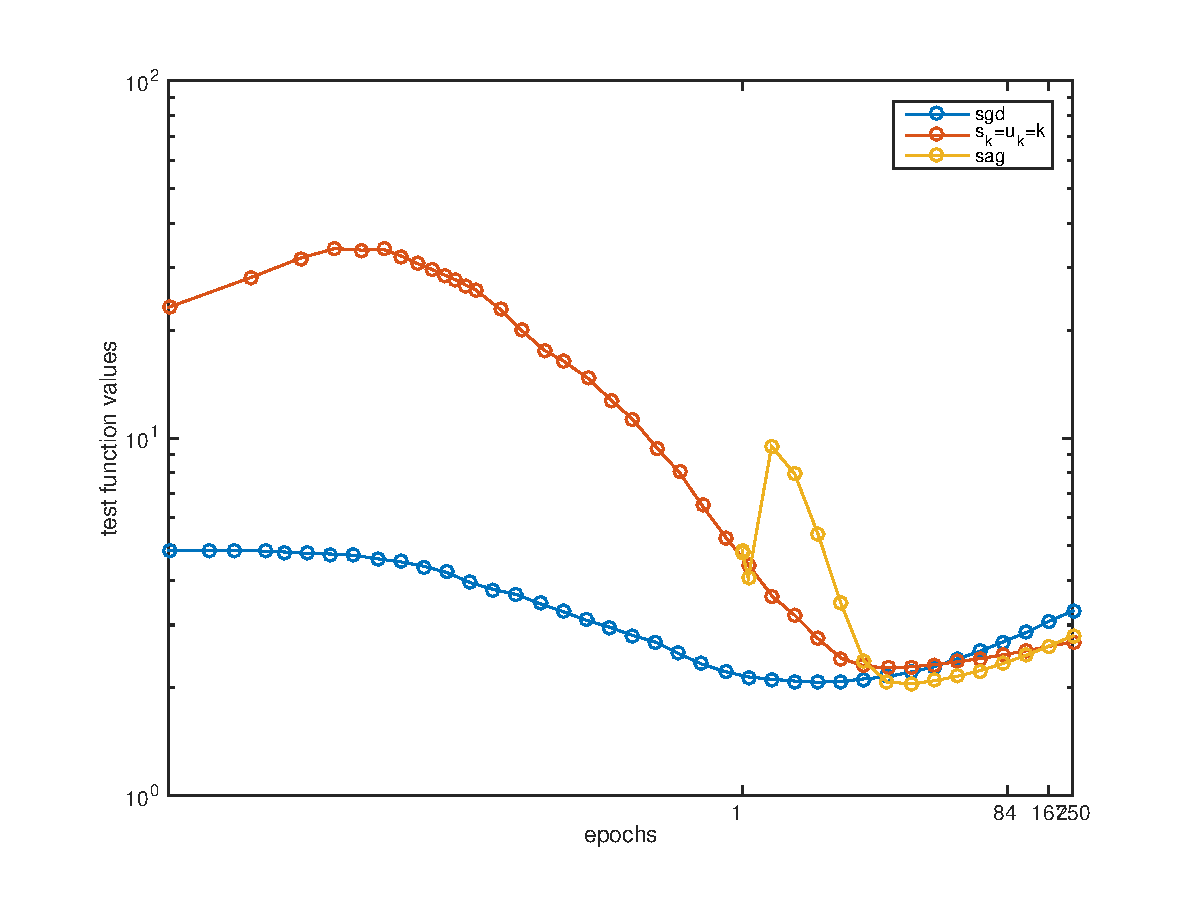
\includegraphics[scale=0.5]{figB.eps}
	\end{center}
\end{frame}
 
		\begin{frame}
			\frametitle{Comments and Conclusions}
			
			ERG:
			\begin{itemize}
	\pause
				\item Competititve with SGD in it's own playing field: in the initial passes through the data
	
	\pause
				\item Has a SAG-like behavior in the later iterations: linear convergence 
	
				\pause
				\item Not only reduces variance, but flexible enough to allow for gradient error to go to zero
	
			\end{itemize}
	
	\pause
			No parameters that depend on the size of the data. Can be run in a truly on-line setting.
	
			\pause
			Theory is in progress
			\begin{itemize}
				\item $F(\theta^k) - \min F(\theta)$ vs $\hat{F}(\theta^k) - \min \hat{F}(\theta)$
			\end{itemize}
			
     	\end{frame}
 

		\begin{frame}
			\frametitle{Questions?}
		\end{frame}
		
\end{document}